\begin{example}
    Требуется доказать
    $$ \fbox{
        $ \forall n \in \N\ \forall x \geq -1: (1 + x)^n \geq 1 + xn $
    } \text{ --- неравенство Бернулли} $$

    Докажем с помощью ММИ
    $$ \forall n \in \N\ \underbrace{\forall x \geq -1\ \underbrace{(1 + x)^n \geq 1 + xn}_{Q(n)}}_{P(n)} $$

    \begin{itemize}
        \item[1)] $ \forall x \geq -1\ (1 + x) \geq 1 + x$ - истина
        \item[2)] Предположим $(1 + x)^{n_0} \geq 1 + xn_0$ - истина. Докажем, что $(1 + x)^{n_0 + 1} \geq 1 + x(n_0 + 1)$:
        
        $$ (1 + x)^{n_0 + 1} \geq 1 + x(n_0 + 1) $$
        $$ (1 + x)^{n_0 + 1} = (1 + x)^{n_0}\underbrace{(1 + x)}_{\geq 0} \geq (1 + x)(1 + xn_0) = $$
        $$ = 1 + x + xn_0 + \underbrace{x^2n_0}_{\geq 0} \geq 1 + x + xn_0 = 1 + x(n_0 + 1) $$
    \end{itemize}
\end{example}

\subsection{Доказательство от противного}
Обозначения: $\overline{A}$ - отрицание к $A$

\begin{example}
    Доказать, что количество простых чисел бесконечно

    Пп (предположим противное). Тогда количество простых чисел конечное число:
    $$ n_1,\ldots,n_k$$
    Рассмотрим следующее число:
    $$ m = n_1\cdot \ldots \cdot n_k+1,\ m \in \N,\ m > n_i\ \forall i = \overline{1, k}\ \text{то есть}\ m \neq n_i\ \forall i = \overline{1, k}$$
    Следовательно, $m$ - составное. Тогда:
    $$ m = n^{\alpha_1}_1 \cdot \ldots \cdot n^{\alpha_k}_k $$
    $$ \exists n_j : m\ \vdots\ n_j $$
    Но $m = n_1\cdot \ldots \cdot n_k+1$ и при делении на $n_i\ \forall i = \overline{1, k}$ дает остаток 1 ($\bot$)
    
    Утверждение доказано
\end{example}

\subsection{Достаточность и необходимость}
\begin{figure}[h]
  \centering
  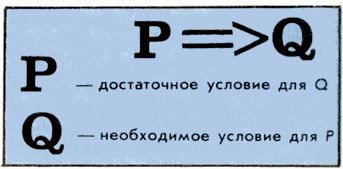
\includegraphics[width=0.5\textwidth]{lectures/files/lec_3_19.09.2025-18-44-35.png}
  \label{fig:lec_3_19.09.2025-18-44-35.png}
\end{figure}

\section{Комбинаторика и Бином Ньютона}
\subsection{Бином Ньютона}

$$ \fbox{
    $ (a + b)^n = \Sum{k = 0}{n} C^k_n a^k b^{n-k} $
} $$

$$ C^0_n a^0 b^{n - 0} + C^1_n a^1 b^{n - 1} + \ldots + C^n_n a^n b^{n - n} $$

где $C^0_n, C^1_n, \ldots $ - биномиальные коэффициенты

\subsection{Комбинаторика}

\begin{definition}
    \textbf{Перестановка} - упорядоченное множество размера $n$ 

    \# перестановок $= n!$
\end{definition}

\begin{definition}
    \textbf{Размещения} - упорядоченное подмножество размера $k$ множества размера $n$

    \# размещений $= \frac{n!}{(n - k)!} = A^k_n$
\end{definition}

\begin{definition}
    \textbf{Сочетания} - неупорядоченное подмножество размера $k$ множества размера $n$

    Одному сочетанию соответствуют $k!$ размещений

    $ \frac{A^k_n}{k!} = \frac{n!}{k!(n-k)!} = C^k_n $
\end{definition}

\section{Последовательности}

\begin{definition}
    \textbf{Последовательность} - индексированный набор чисел

    $ \{a_n\}_{n \in \N} $
\end{definition}

\subsection{Способы задания последовательности}
\begin{itemize}
    \item[1)] Формульный $a_n = n^2 + n - 7$
    \item[2)] Рекуррентный $a_1 = 1, a_2 = 1, a_n = a_{n-1} + a_{n-2} $
\end{itemize}

\begin{definition}
    Последовательность называется \textbf{ограниченной}, если
    $$ \fbox{
        $ \exists c\ \forall n\ |a_n| \leq c $
    } = P(\{a_n\}) $$
    И \textbf{неограниченной}, если
    $$ \fbox{
        $ \forall c\ \exists n(c)\ |a_{n(c)}| > c $
    } $$
\end{definition}

\begin{example}
    $$ a_n = \frac{3n^2 + 5n - 2}{2n^2 + n + 1} $$
    $$ \l|\frac{3n^2 + 5n - 2}{2n^2 + n + 1}\r| \leq \l|\frac{3n^2 + 5n^2}{2n^2}\r| \leq \l|\frac{8n^2}{2n^2}\r| \leq c $$
    $$ 4 \leq c $$
    $$ \exists c = \pi^2\ \forall n\ \l|\frac{3n^2 + 5n - 2}{2n^2 + n + 1}\r| \leq c$$
\end{example}
